






\section{Evaluation}
\label{sec:eval}

We evaluate Hector with the following questions to answer.


\begin{enumerate}[Q1.]
\item How does the performance of Hector compare with state-of-the-art systems? How does Hector achieve it?
\item How much improvement do the two optimizations detailed in \cref{sec:materialization,sec:inter_op_opt}, compaction materialization and linear operator reordering, make? 
\item Any architectural insights for GPU for RGNNs?
\end{enumerate}



\cref{sec:baseline_eval} answers Q1. \cref{sec:dse_eval} answers Q2 and further analyzes the performance implications of the two optimizations through a case study. \cref{sec:arch_analysis} addresses Q3.


\begin{table}[!htbp]
\centering
\begin{tabular}{lll|lll}
\toprule
\textbf{Name} & \multicolumn{1}{l}{\textbf{\begin{tabular}[c]{@{}l@{}}\#\ nodes\\(\#\ types)\end{tabular}}} & \multicolumn{1}{l|}{\textbf{\begin{tabular}[c]{@{}l@{}}\#\ edges\\(\#\ types)\end{tabular}}}  & \textbf{Name} & \multicolumn{1}{l}{\textbf{\begin{tabular}[c]{@{}l@{}}\#\ nodes\\(\#\ types)\end{tabular}}} & \multicolumn{1}{l}{\textbf{\begin{tabular}[c]{@{}l@{}}\#\ edges\\(\#\ types)\end{tabular}}}    \\ \midrule
aifb                           & 7.3K~(7)    & 49K~(104) & fb15k                           & 15K~(1)  & 620K~(474) \\ 
am                           & 1.9M~(7) & 5.7M~(108) & mag                           & 1.9M~(4) & 21M~(4) \\ 
bgs                              & 95K~(27)   & 673K~(122)&  mutag                          & 27K~(5)   & 148K~(50) \\     
biokg                           & 94K~(5)   & 4.8M~(51)&   wikikg2                     & 2.5M~(1) & 16M~(535) \\ \bottomrule 
\end{tabular}
\caption{Heterogeneous graph datasets~\cite{aifb, mutag, bgs, am, huOpenGraphBenchmark2021, toutanovaObservedLatentFeatures2015} used in our evaluation. The numbers reflect the default preprocessing by the OGB and DGL packages, e.g., adding inverse edges.}\label{tab:datasets}
\end{table}


\subsection{Experimental Setup}
\label{sec:eval_methodology}

To assess performance, we measure the inference and training time of Hector and other systems on a single-GPU computer. Its hardware components include one Intel Core i9-9900K CPU, 128 GB dual-channel memory, and one Nvidia RTX 3090 GPU with 24 GB memory. The operating system is Ubuntu 18.04.5, with kernel version 5.4.0-135. The CUDA and driver versions are 12.1 and 530.30.02, respectively. PyTorch and DGL versions are 2.0.1 and 1.1.1, respectively.


As shown in Table~\ref{tab:datasets}, we use public datasets from DGL~\cite{wang2019deep} and OGB~\cite{huOpenGraphBenchmark2021}.
We measure (1)~inference and (2)~training time on three RGNN models,  RGCN~\cite{rgcn}, RGAT~\cite{busbridge2019relational}, and HGT~\cite{hgt}, comparing with previous systems, involving DGL~\cite{wang2019deep}, PyG~\cite{fey2019fast}, Seastar~\cite{wuSeastarVertexcentricProgramming2021}, Graphiler~\cite{xieGraphilerCompilerGraph}, and HGL~\cite{guiHGLAcceleratingHeterogeneous}.
We ported Seastar artifacts to the same version of CUDA and Python packages as Hector depends on because one of Seastar's dependencies, dgl 0.4, used an API deprecated since CUDA~11.


For RGCN, RGAT, and HGT, excluding comments, Hector took in 51 lines in total and produced more than 3K lines of CUDA kernel code, 5K lines of other C++ code to define host functions, and 2K lines of Python code to define subclasses of PyTorch \texttt{autograd.Function}. The implementation also involves 2K lines of Python code providing common utilities. 


To best align with the hyper-parameters prior work used in its evaluation, we set the input and output feature dimensions as 64 and the number of heads as 1. 
We measure the inference and training time of the single layer used. 
In training, to obtain a loss, we compute the negative log-likelihood loss by comparing the output with a precomputed random label tensor. 
For each case, we run the full graph inference and training for at least 10 epochs and average the elapsed time.
To align with the existing system, nodes are presorted to enable segment MM for typed linear layers.



\subsection{Comparison with Prior Work}
\label{sec:baseline_eval}


For the performance of DGL and PyG, we measure all public implementations of these models from DGL, PyG, and Graphiler artifacts.
PyG provides two RGCN convolution layers: \texttt{RGCNConv} places nodes in segments of the same type but launches separate kernels for each of the node types, leading to device underutilization.
\texttt{FastRGCNConv} replicates weights and uses \texttt{bmm()}. It is consistently faster than the \texttt{RGCNConv} implementation.
Similarly, DGL's built-in segmentMM-based RGCN layer is faster than other DGL implementations.
For HGT, the DGL segmentMM-based \texttt{HGTConv} primitive generally has the best performance.
In the cases where some variants encounter OOM errors, we choose the best among those that run without issues.
Some cases are missing due to insufficient operator support, such as HGL on HGT and Graphiler on training. We do not measure HGL in inference because it is designed to optimize training.



Figure~\ref{fig:inference_results} shows that Hector's best-optimized code consistently outperforms state-of-the-art systems. It achieves up to 9.9$\times$ speed-up in inference and up to 43.7$\times$ speed-up in training against the best state-of-the-art systems. On geometric average, Hector gets 1.79$\times$, 8.56$\times$, 2.87$\times$ speed-up in inference via RGCN, RGAT, and HGT, respectively, and 2.59$\times$, 11.34$\times$, 8.02$\times$ speed-up in training RGCN, RGAT, and HGT, respectively. The performance advantage is larger in small graphs, demonstrating that \textbf{generating a single kernel that performs the computation across multiple edge types boosts the performance on small graphs %
compared to existing systems that run many small kernels}. 



\begin{figure}[!htbp]\captionsetup[subfigure]{font=small}
\centering
\subcaptionbox{Training time}
[\linewidth]{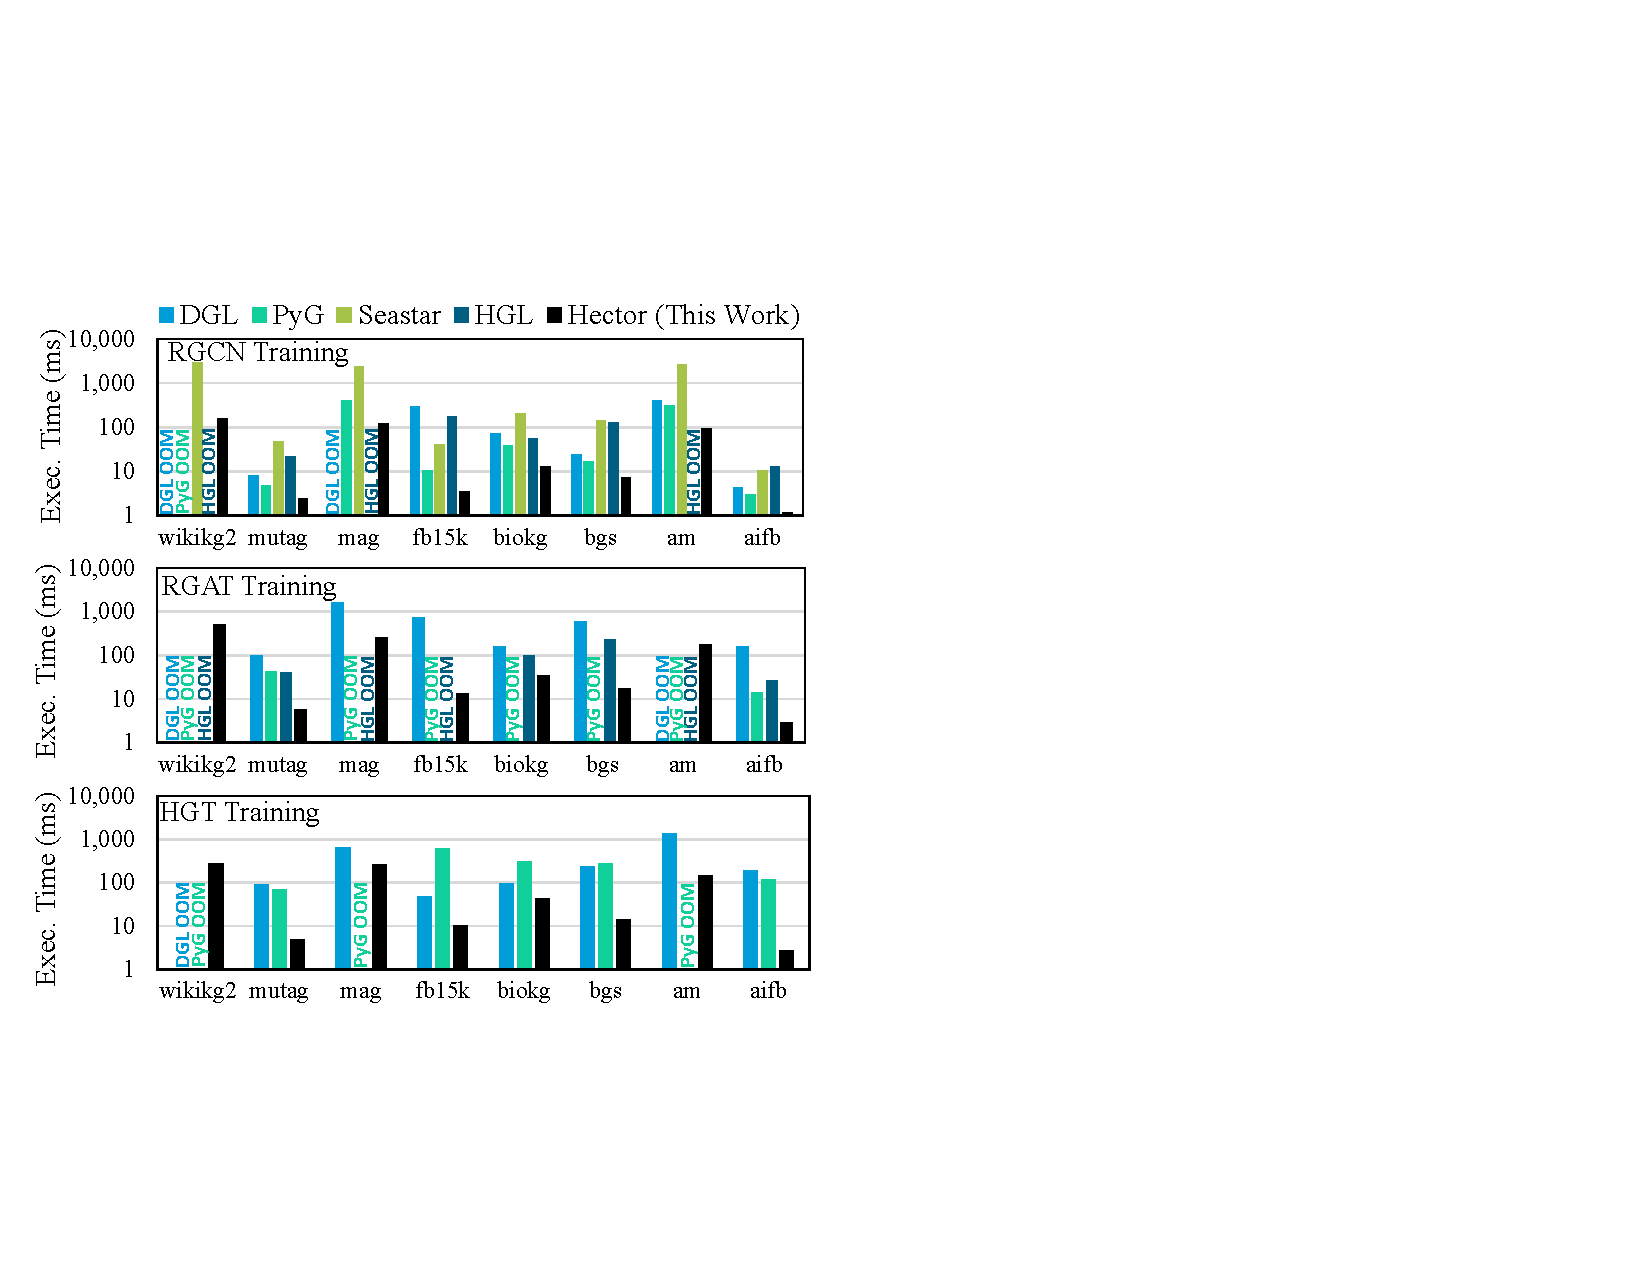
\includegraphics[scale=0.8]{figures/Hector/training_time_final.pdf}}
\subcaptionbox{Inference time}
[\linewidth]{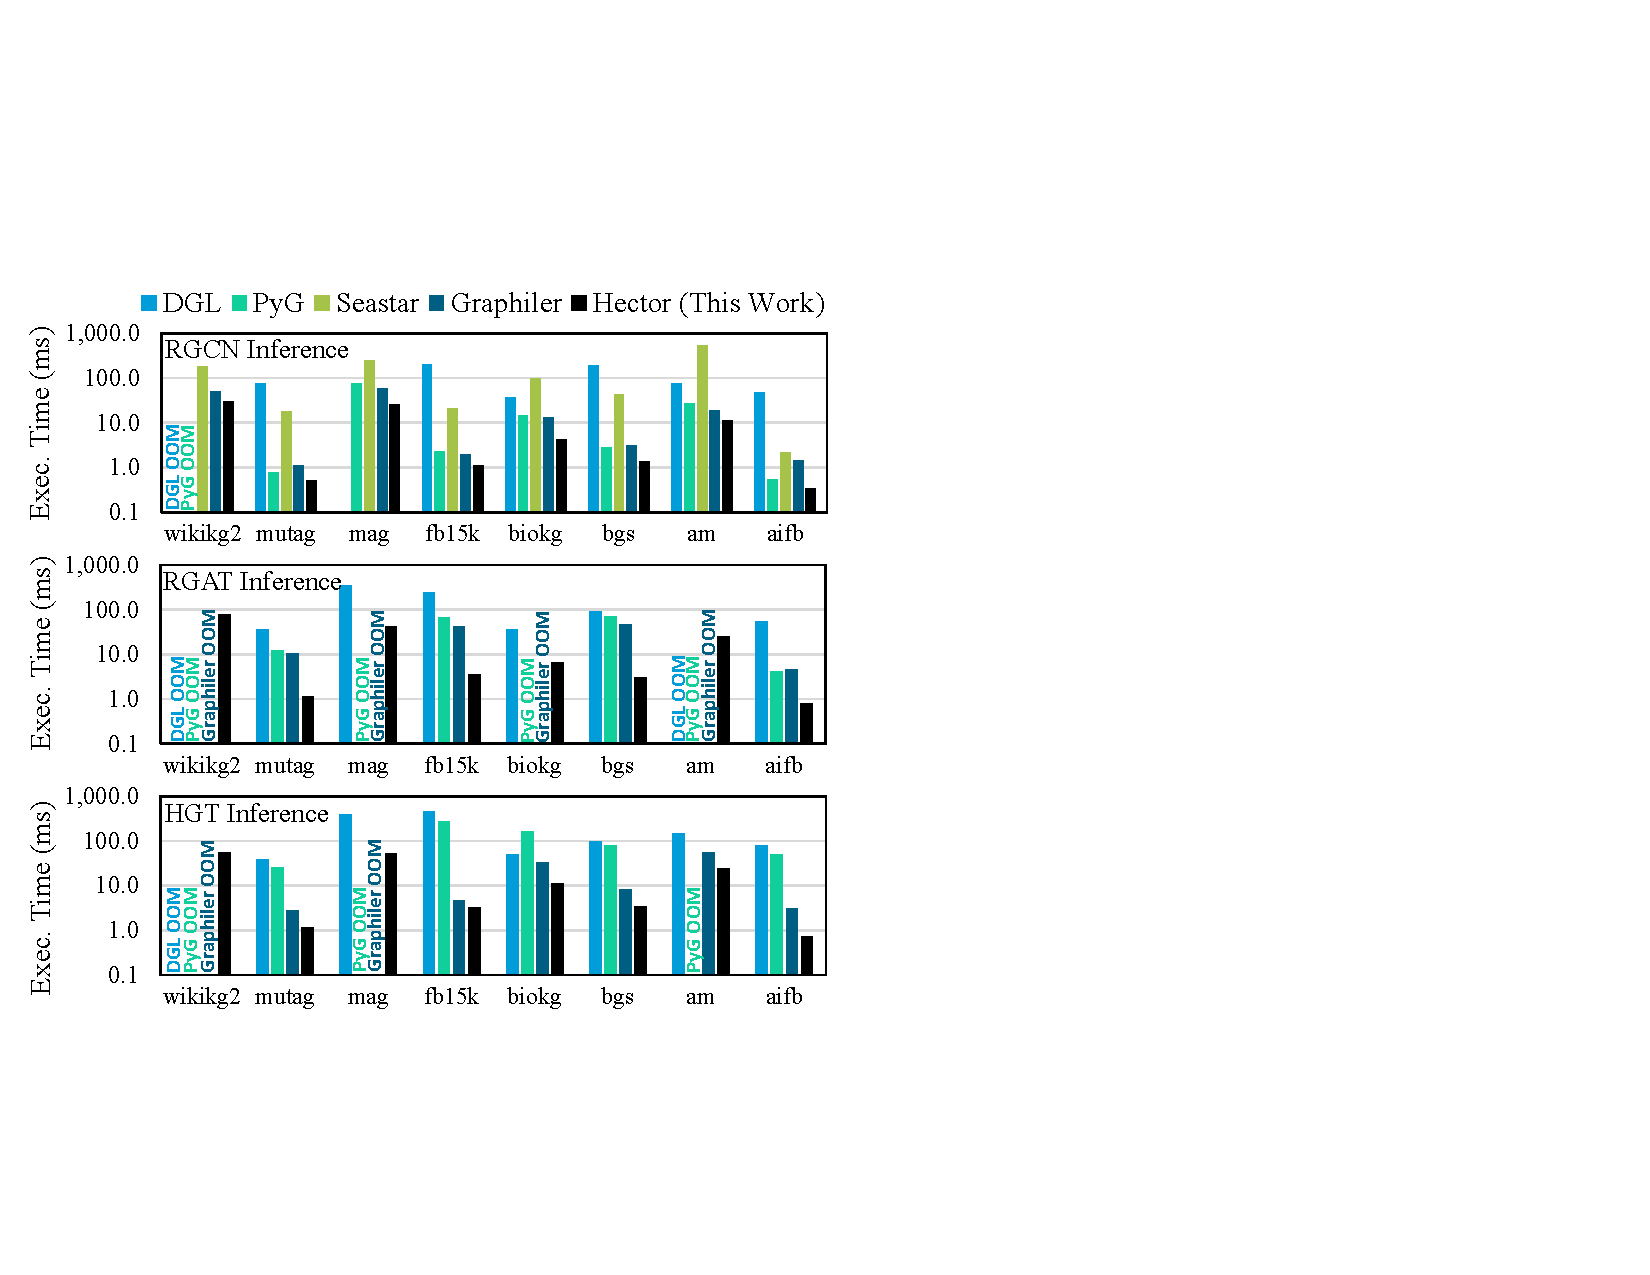
\includegraphics[scale=0.8]{figures/Hector/inference_time_final.pdf}}
\caption{\label{fig:inference_results} Comparing the execution~(Exec.) time of Hector best optimized code with previous work. Table~\ref{tab:datasets} shows the datasets used. }
\end{figure}

We see close performance achieved by Graphiler in RGCN and HGT inference. Graphiler leverages PyTorch utilities to produce TorchScript binaries before execution and utilizes edgewise parallelism for edgewise computation. Similarly to \texttt{RGCNConv}, it places node features into segments of the same type but runs separate kernels to perform a typed linear transformation. DGL and PyG, under similar configurations, achieve competitive performance. However, when it comes to RGAT, Graphiler suffers from performance degradation. Because Graphiler relies on pre-programmed fused kernels to deliver a significant portion of the performance boost~\cite{xieGraphilerCompilerGraph}, we postulate that the degradation is due to the non-exhaustiveness of these pre-programmed kernels~\cite{xieGraphilerRepositoryGithub2023}.
This reflects the drawbacks of compiler design without a code generation mechanism. By contrast, with two-level IR and a code generator, Hector achieves better performance, showing that \textbf{generating kernels with flexible access scheme that gather and scatter data on the fly eliminates redundant data movement and outperforms indexing/copying followed by hand-optimized GEMM and sparse kernels}. Besides, it is challenging to extend Graphiler's approach to training due to TorchScript's limited auto-differentiation support. For example, \texttt{dict} object creation is not supported, but it is a common way to express nodewise and edgewise data. 

By comparing Hector with Seastar, which lowers all logic to sparse kernels, we realize that \textbf{sparse kernel code generation alone is not efficient in RGNNs: it is better to lower to GEMM kernels as much as possible}.





There are two reasons why Hector is more efficient in device memory usage. First, Hector only keeps a single copy of weights, as discussed in Section~\ref{sec:materialization}. Replicating weights also affects backward propagation because the gradient of each copy will be derived, occupying extra memory. Second, our compact materialization reduces memory and redundant computation, as explained in Section~\ref{sec:dse_eval}.








Notably, even without compact materialization or linear operator reordering, Hector still consistently outperforms existing systems, as Table~\ref{tab:base_vs_baseline} shows. In addition, the unoptimized Hector code triggers fewer OOMs than existing systems, with the only exception where the RGAT inference is run on mag and wikikg2. 
For comparison, we also show the statistics of the best optimized Hector code in Table~\ref{tab:base_vs_baseline}.


\begin{table}[!htbp]
\centering
\begin{tabular}{lllllc|lllc}
 \toprule
&     & \multicolumn{4}{c}{\textbf{Training}}               & \multicolumn{4}{c}{\textbf{Inference}}              \\
&     & \multicolumn{1}{l}{\textbf{W}} & \textbf{M} & \textbf{B} & \multicolumn{1}{l}{\textbf{\#E}}  & \textbf{W} & \textbf{M} & \textbf{B} & \textbf{\#E}\\ \midrule
\multirow{3}{*}{\rotatebox[origin=c]{90}{\textbf{unopt.}}}& RGCN & 2.02 & 2.59 & 3.47  & \underline{0} & 1.51 & 1.79 & 2.19 & \underline{0} \\
& RGAT & 1.72 & 9.14 & 43.7 & \underline{2} & 1.41 & 5.02 & 9.89 & \underline{2} \\
& HGT  & 1.53 & 6.62 & 28.3 & \underline{0} & 1.20 & 1.90 & 4.31 & \underline{0} \\\hline
\multirow{3}{*}{\rotatebox[origin=c]{90}{\textbf{b.\ opt.}}}& RGCN & 2.02 & 2.76 & 3.48  & \underline{0} & 1.51 & 1.91 & 3.20 & \underline{0} \\
& RGAT & 4.61 & 11.3 & 55.4 & \underline{0} & 5.29 & 8.56 & 15.5 & \underline{0} \\
& HGT  & 2.17 & 8.02 & 43.1 & \underline{0} & 1.40 & 2.87 & 7.42 & \underline{0} \\
\bottomrule
\end{tabular}
\caption{Comparing to the best in state-of-the-art systems, speed-ups of Hector unoptimized~(unopt.) code and that of Hector best optimized~(b.\ opt.) code. Worst~(W), average~(M), and best~(B) cases. Numbers of OOMs Hector triggers~(\#E) are shown. \label{tab:base_vs_baseline}}
\end{table}








\subsection{Effects of Compact Materialization and Linear Operator Reordering}
\label{sec:dse_eval}
Now, we study the effects of compact materialization and linear operator reordering. They are detailed in \cref{sec:materialization,sec:inter_op_opt}. 
We investigate their effects on RGAT and HGT.



Table~\ref{tab:optimizations} shows the speed-up on top of Hector unoptimized code by these two optimizations. Due to compact materialization, Hector no longer triggers OOM errors when running RGAT on mag and wikikg2. In addition, in some cases, the layout speeds up the execution due to the common subexpression elimination brought forth by the layout. Compact materialization is hardly possible without a code generation scheme or an IR design that decouples the model semantics, data layout, and operator-specific schedule.
Besides, \textbf{data layout choice, compact materialization, in particular, allows further performance enhancement} while prior work usually focuses on improving the schedule given a specific sparse matrix format. This is shown by the significant speed-ups in the ``C[ompact]'' columns in Table~\ref{tab:optimizations}.



\begin{table}[htbp!]
\centering
\begin{tabular}{clccc|ccc} 
\toprule
\multicolumn{2}{l}{\multirow{2}{*}{\textbf{}}} & \multicolumn{3}{c}{\textbf{Training}}                                                                                          & \multicolumn{3}{c}{\textbf{Inference}}                                                                                          \\
\multicolumn{2}{l}{}                           & \multicolumn{1}{l}{\textbf{C}}           & \textbf{R}                               & \multicolumn{1}{c}{\textbf{C+R}}         & \textbf{C}                               & \textbf{R}                               & \textbf{C+R}                              \\ 
\midrule
\multirow{9}{*}{\rotatebox[origin=c]{90}{RGAT}}  & aifb    & \cellcolor[HTML]{D97460}0.80 & \cellcolor[HTML]{EEF4EC}\textbf{1.14}           & \cellcolor[HTML]{E08E7D}0.84          & \cellcolor[HTML]{FEFFFE}1.01          & \cellcolor[HTML]{E9F0E6}\textbf{1.19}           & \cellcolor[HTML]{F3F7F1}1.10          \\
 & am      & \cellcolor[HTML]{F2D1CB}0.94 & \cellcolor[HTML]{F2F6F0}\textbf{1.12}                    & \cellcolor[HTML]{FDF8F7}{0.99} & \cellcolor[HTML]{DAE6D5}1.31          & \cellcolor[HTML]{DEE8D9}1.28                    & \cellcolor[HTML]{C0D4B7}\textbf{1.54} \\
 & bgs     & \cellcolor[HTML]{F2D0C9}0.93 & \cellcolor[HTML]{EAF0E7}\textbf{1.18}           & \cellcolor[HTML]{FBFCFA}{1.04} & \cellcolor[HTML]{DDE8D9}1.29          & \cellcolor[HTML]{D7E4D2}{1.34}           & \cellcolor[HTML]{BCD1B3}\textbf{1.57} \\
 & biokg   & \cellcolor[HTML]{39771E}2.67 & \cellcolor[HTML]{E1EADD}1.26                    & \cellcolor[HTML]{38761D}\textbf{2.68} & \cellcolor[HTML]{38761D}\textbf{3.76} & \cellcolor[HTML]{D0DFC9}1.40                    & \cellcolor[HTML]{38761D}{3.74} \\
& fb15k & \cellcolor[HTML]{E8EFE5}1.20 & \cellcolor[HTML]{E7EFE4}1.20 & \cellcolor[HTML]{E0EADB}\textbf{1.27} & \cellcolor[HTML]{C5D7BD}1.50 & \cellcolor[HTML]{E1EADD}1.26 & \cellcolor[HTML]{B6CDAC}\textbf{1.62} \\
 & mag     & \cellcolor[HTML]{C3D6BB}1.51 & \multicolumn{1}{l}{\cellcolor[HTML]{F9FBF8}OOM} & \cellcolor[HTML]{BCD1B3}\textbf{1.57} & \cellcolor[HTML]{FFFFFF}1.00*          & \multicolumn{1}{l}{\cellcolor[HTML]{F3F7F2}OOM} & \cellcolor[HTML]{F8FAF7}\textbf{1.07} \\
 & mutag   & \cellcolor[HTML]{CC4125}0.70 & \cellcolor[HTML]{EFF4ED}\textbf{1.14}           & \cellcolor[HTML]{CC4125}0.73          & \cellcolor[HTML]{E4EDE0}1.23          & \cellcolor[HTML]{E3ECE0}{1.24}           & \cellcolor[HTML]{D5E2CF}\textbf{1.36} \\
 & wikikg2 & \cellcolor[HTML]{F4F8F3}1.09 & \multicolumn{1}{l}{\cellcolor[HTML]{F7FAF6}OOM} & \cellcolor[HTML]{F1F6EF}\textbf{1.12} & \cellcolor[HTML]{FFFFFF}1.00*          & \multicolumn{1}{l}{\cellcolor[HTML]{EDF3EB}OOM} & \cellcolor[HTML]{FEFEFD}\textbf{1.02} \\
 & AVERAGE & \cellcolor[HTML]{F0F5EE}1.13 & \cellcolor[HTML]{EBF1E8}1.17                    & \cellcolor[HTML]{EAF1E7}\textbf{1.18} & \cellcolor[HTML]{D5E2CF}1.36          & \cellcolor[HTML]{DEE8D9}1.28                    & \cellcolor[HTML]{C6D8BE}\textbf{1.49}
                  \\ 
\hline
\multirow{9}{*}{\rotatebox[origin=c]{90}{HGT}} & aifb    & \cellcolor[HTML]{F9E8E5}0.97 & \cellcolor[HTML]{C2D5B9}\textbf{1.52} & \cellcolor[HTML]{D1DFCA}1.40          & \cellcolor[HTML]{F0C9C1}0.92 & \cellcolor[HTML]{90B381}\textbf{1.94} & \cellcolor[HTML]{BBD0B1}1.58          \\
& am      & \cellcolor[HTML]{FAFCF9}1.05 & \cellcolor[HTML]{F1F6EF}1.12          & \cellcolor[HTML]{E9F0E6}\textbf{1.19} & \cellcolor[HTML]{F9FBF8}1.06 & \cellcolor[HTML]{DAE6D5}1.32          & \cellcolor[HTML]{CEDDC7}\textbf{1.42} \\
& bgs     & \cellcolor[HTML]{FEFCFB}1.00* & \cellcolor[HTML]{F2F6F0}1.11          & \cellcolor[HTML]{EAF1E8}\textbf{1.18} & \cellcolor[HTML]{F3D5CF}0.94 & \cellcolor[HTML]{E1EBDD}\textbf{1.25} & \cellcolor[HTML]{E3ECDF}1.24          \\
& biokg   & \cellcolor[HTML]{D6E3D1}1.35 & \cellcolor[HTML]{FCFDFB}1.03          & \cellcolor[HTML]{CFDEC8}\textbf{1.41} & \cellcolor[HTML]{CBDBC4}1.45 & \cellcolor[HTML]{F8FAF6}1.07          & \cellcolor[HTML]{BBD0B2}\textbf{1.58} \\
& fb15k   & \cellcolor[HTML]{E7A79A}0.88 & \cellcolor[HTML]{F2F6F0}\textbf{1.11} & \cellcolor[HTML]{F8E5E2}0.96          & \cellcolor[HTML]{D35E46}0.77 & \cellcolor[HTML]{ECF2EA}\textbf{1.16} & \cellcolor[HTML]{E59F91}0.86          \\
& mag     & \cellcolor[HTML]{E3ECDF}1.24 & \cellcolor[HTML]{F9FBF8}1.06          & \cellcolor[HTML]{D7E4D2}\textbf{1.34} & \cellcolor[HTML]{C9DAC1}1.46 & \cellcolor[HTML]{F3F7F2}1.10          & \cellcolor[HTML]{AAC59F}\textbf{1.72} \\
& mutag   & \cellcolor[HTML]{FEFDFD}1.00 & \cellcolor[HTML]{D9E5D4}\textbf{1.32} & \cellcolor[HTML]{DAE6D5}1.32          & \cellcolor[HTML]{F4D7D1}0.94 & \cellcolor[HTML]{AFC8A4}\textbf{1.68} & \cellcolor[HTML]{C4D6BC}1.50          \\
& wikikg2 & \cellcolor[HTML]{E6EEE2}1.22 & \cellcolor[HTML]{F7FAF6}1.07          & \cellcolor[HTML]{D8E5D3}\textbf{1.33} & \cellcolor[HTML]{E1EBDD}1.26 & \cellcolor[HTML]{EDF3EB}1.15          & \cellcolor[HTML]{C3D6BB}\textbf{1.51} \\
& AVERAGE & \cellcolor[HTML]{F6F9F5}1.08 & \cellcolor[HTML]{ECF2EA}1.16          & \cellcolor[HTML]{E1EADD}\textbf{1.26} & \cellcolor[HTML]{F7F9F5}1.07 & \cellcolor[HTML]{DBE6D6}1.31          & \cellcolor[HTML]{D0DFCA}\textbf{1.40}
        \\
\bottomrule
\end{tabular}
\begin{flushleft} \footnotesize *Normalized by the performance with compact materialization~(C) because the unoptimized version triggers OOM errors. 
\end{flushleft}
\caption{Speed-up on top of Hector unoptimized code due to compaction~(C) and linear operator reordering~(R). Input and output dimensions are both 64. The highest speed-ups per task are in bold. }
\label{tab:optimizations}
\end{table}

To study how compact materialization reduces the memory footprint, we illustrate the Hector DRAM usage without compact materialization in Figure~\ref{fig:dram_analysis}(b) and the portion of DRAM usage with compact materialization in Figure~\ref{fig:dram_analysis}(a). For simplicity, we define the entity compaction ratio as the number of unique $(\text{source node}, \text{edge type})$ pairs divided by the number of edges. Figure~\ref{fig:dram_analysis}(b) shows that the memory use of inference and training is highly proportional to the number of edges of the datasets. Figure~\ref{fig:dram_analysis}(a) shows that compact materialization significantly reduces DRAM usage in all datasets. The memory footprint ratio of compact materialization compared with the memory footprint of the unoptimized code correlates with the entity compaction ratio. The memory footprint ratio is higher than the entity compaction ratio, as the memory footprint consists of edgewise data, nodewise data, and weights, whereas the compaction applies to edgewise data only. Besides, in case the average degrees are larger, the memory footprint ratio reduces more significantly, getting closer to the entity compaction ratio.


\begin{figure}[!htbp]
\centering
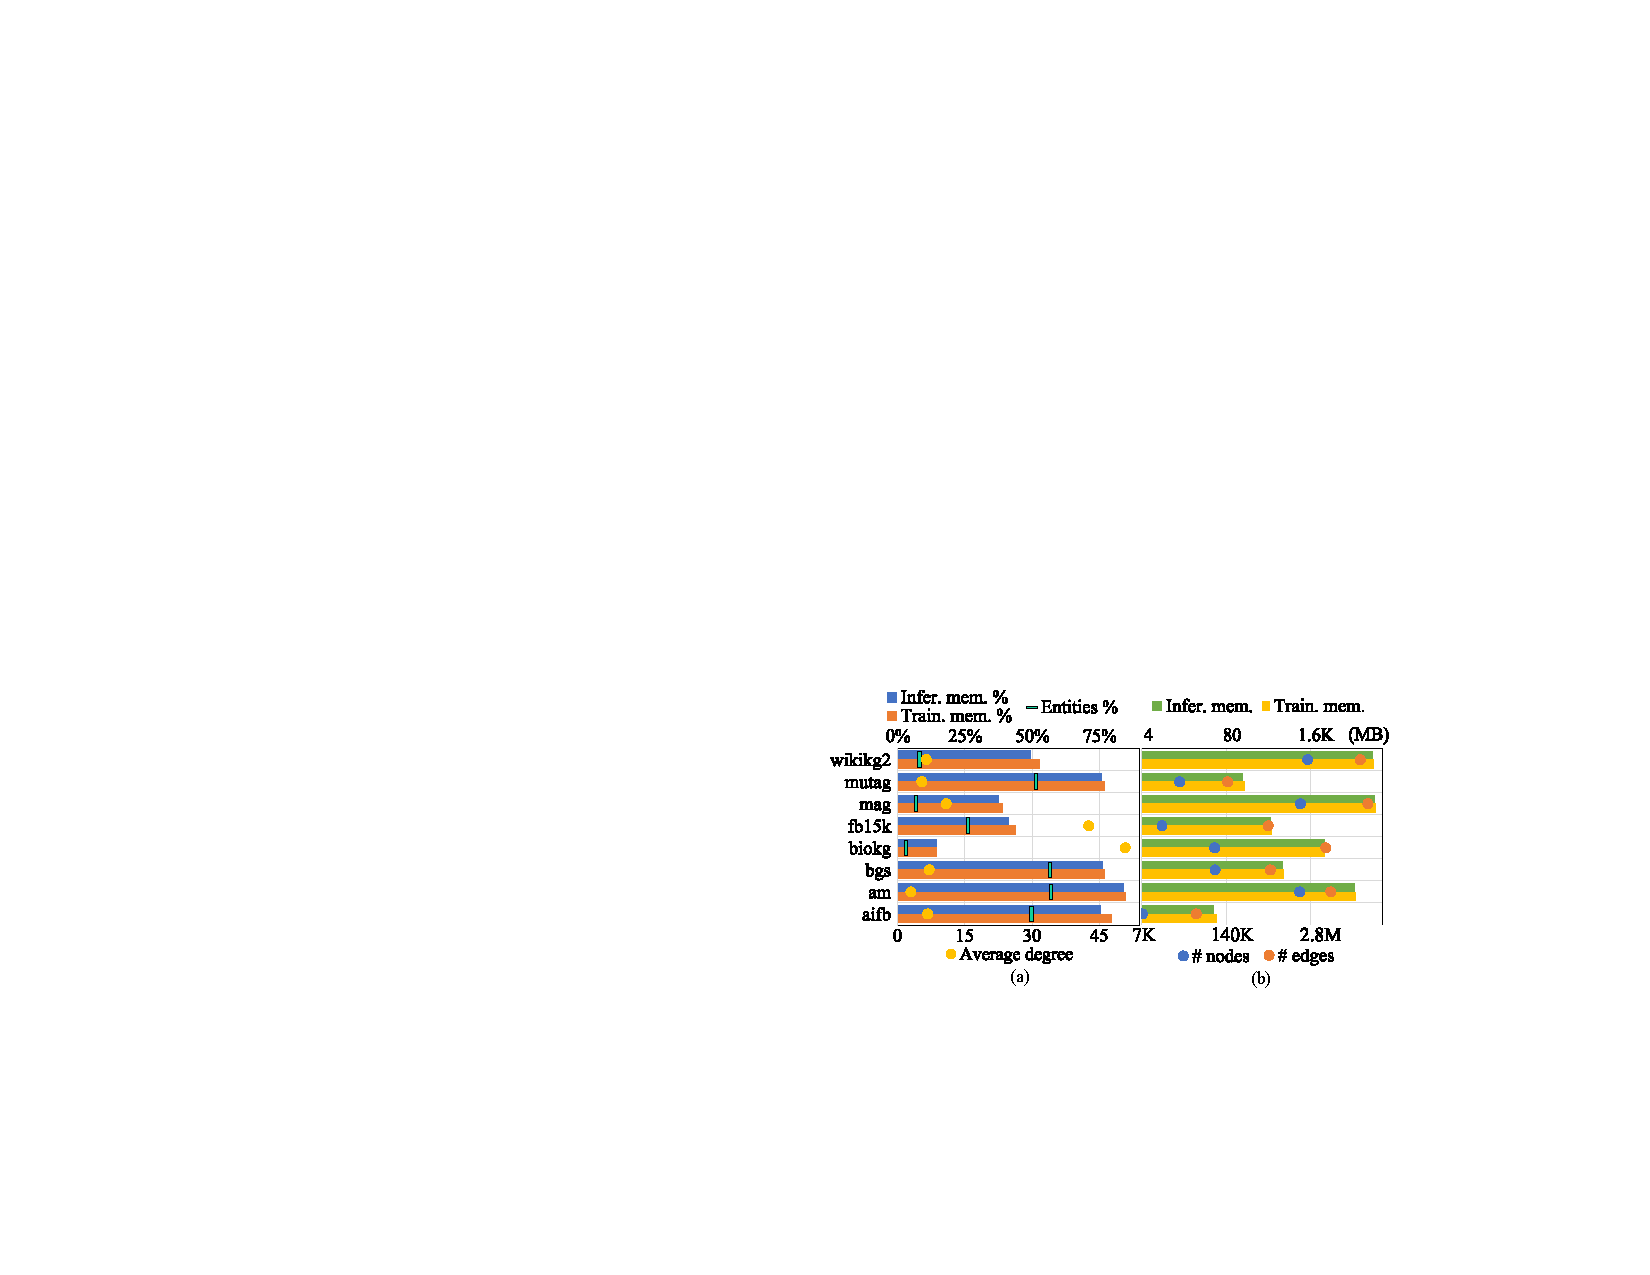
\includegraphics[width=\linewidth]{figures/Hector/DRAMAnalysis_v2.3.pdf}
\caption{\label{fig:dram_analysis} Memory usage when Hector runs training and inference on HGT. (b) shows the inference memory use~(Infer.\ mem.) and training memory use~(Train.\ mem.) of the unoptimized Hector code in MBs. (a) shows the portion of the memory use after applying compact materialization vs. the unoptimized Hector code. For comparison, the number of nodes~(\#\ nodes), number of edges~(\#\ edges), and average degree of datasets are shown as dot scatters. The entity compaction ratio of each dataset is also shown. Legend entries of each data series are placed next to the series' axis.}
\end{figure}


To better understand the performance benefits of optimizations, Figure~\ref{fig:perf_analysis} studies two cases. 
The entity compaction ratio of AM and FB15k are 57\% and 26\%, respectively. On AM, the time GEMM instances take is greatly reduced. By comparison, in FB15k, compaction brings less performance improvement due to the less significant GEMM reduction. 


\begin{figure}[!htbp]
\centering
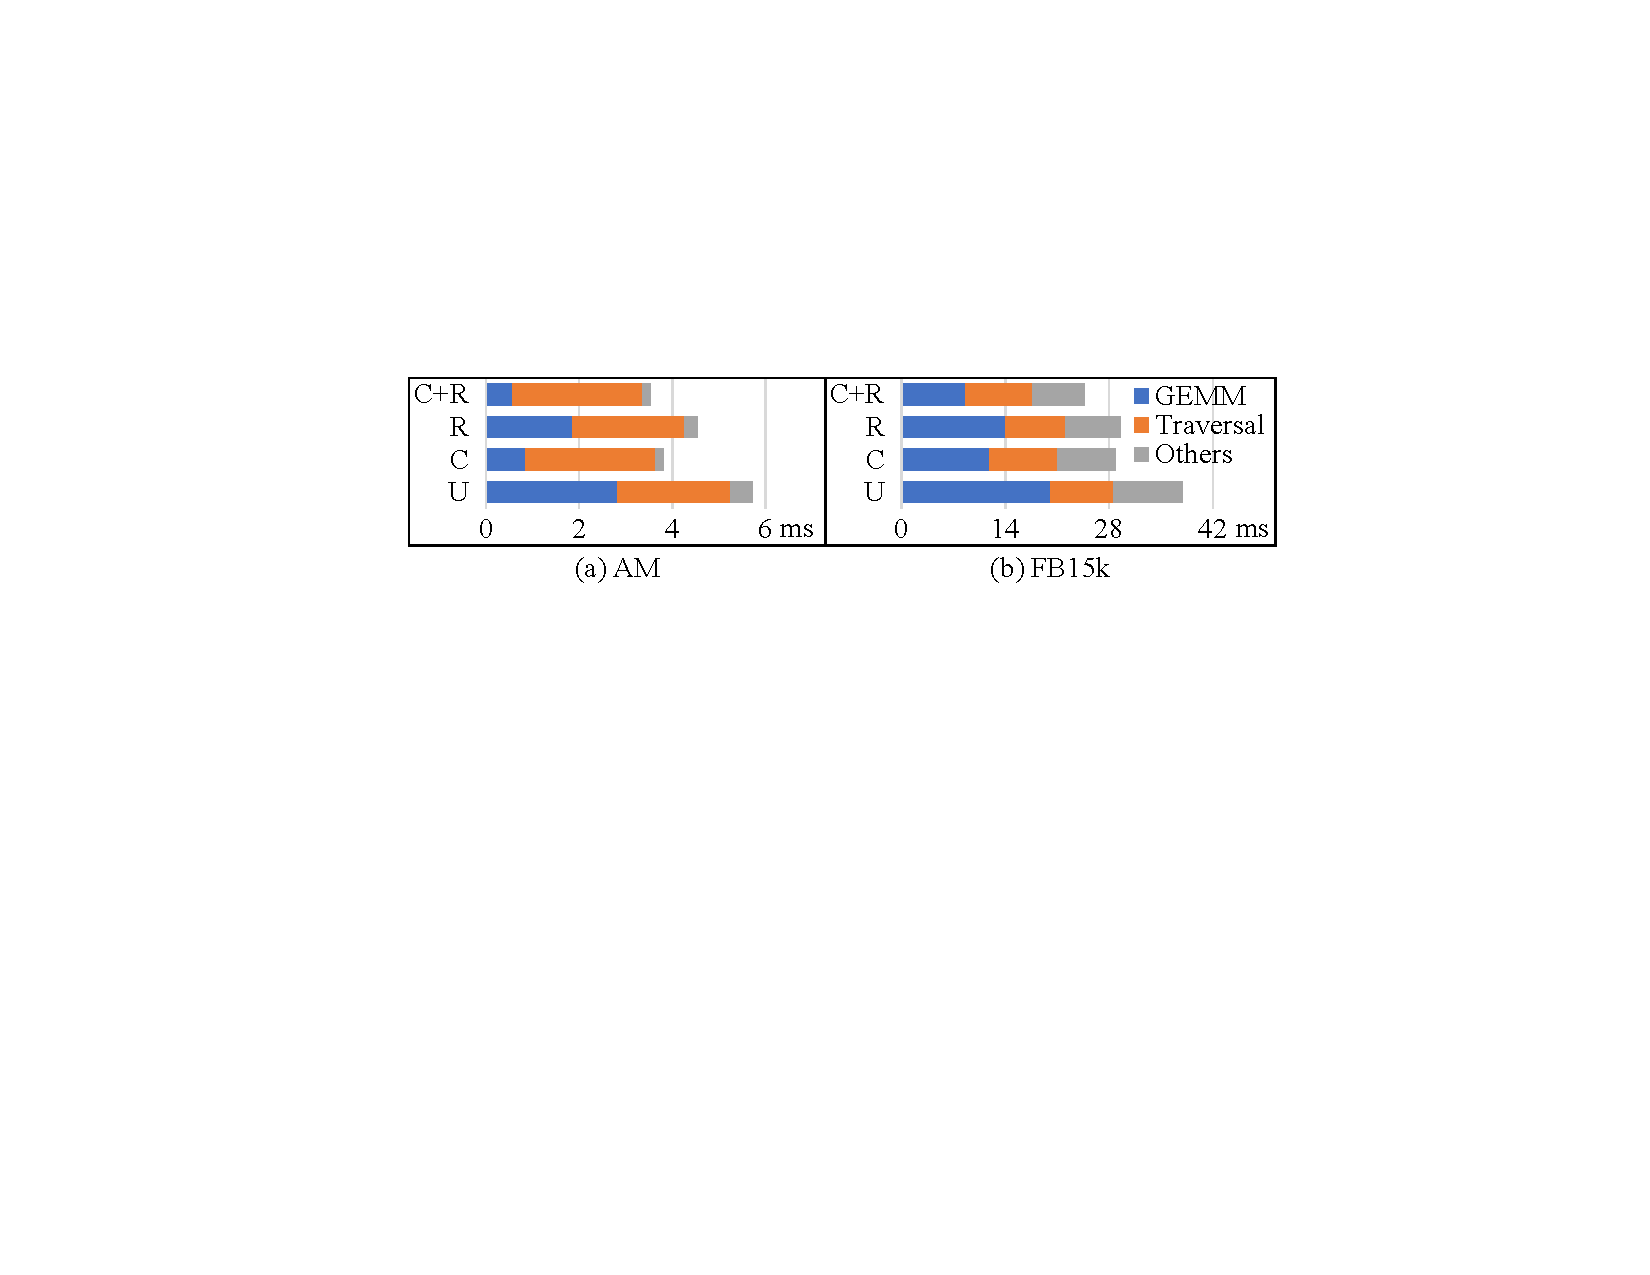
\includegraphics[width=
\linewidth]{figures/Hector/FB15K.AM.BreakdownEvalv3.compact.pdf}
\caption{\label{fig:perf_analysis} Breakdown of Hector RGAT inference on two datasets. Input and output dimensions are 64. Cases with compaction~(C), linear operator reordering~(R), and no optimization~(U) are presented.}
\end{figure}

In short, \textbf{due to the data-dependent nature of computation in RGNNs, there is no one-size-fits-all optimization strategy}. However, as shown in Table~\ref{tab:optimizations}, enabling compaction and reordering obtains fairly good performance consistently and is the best fixed strategy on average in all four scenarios, i.e., $\{\text{RGAT}, \text{HGT}\}\times\{\text{training},\text{inference}\}$. If Hector presumably chooses the best configuration in every run, it could further get 1.06$\times$, 1.33$\times$, 1.02$\times$, and 1.08$\times$ speed-up in the four scenarios above, respectively. We leave autotuning to future work.






\subsection{Analyzing the Architectural Characteristics}
\label{sec:arch_analysis}

We show the average time of unoptimized Hector in Figure~\ref{fig:perf_curve}. We also profile generated kernels when running Hector on RGAT on bgs and am, as shown in Figure~\ref{fig:arch_number}.






One thing to note is the sublinear time increase in Figure~\ref{fig:perf_curve}: when the input and output dimension doubles, the amount of computation and memory accesses becomes close to 4$\times$ those of the original, but the time increase is typically lower than 2$\times$ of the original. The reason is increased computation throughput when the size increases, as corroborated by Figure~\ref{fig:arch_number}. Moreover, we observed higher throughput when the graph scale increases, e.g., from bgs to am in Figure~\ref{fig:arch_number}. Similarly, we witnessed the cuBLAS throughput increases steadily when we keep the right matrix size as (64, 64) and increase the number of rows of the left matrix from 1M~(2\textsuperscript{17}) to 8M~(2\textsuperscript{20}). These suggest that \textbf{an RGNN system should be memory-efficient in order to accommodate larger models and datasets to fully utilize the massive resources on GPUs}. By eliminating unnecessary data copies, Hector achieves better memory efficiency than state-of-the-art systems.



\begin{figure}[!htbp]
\centering
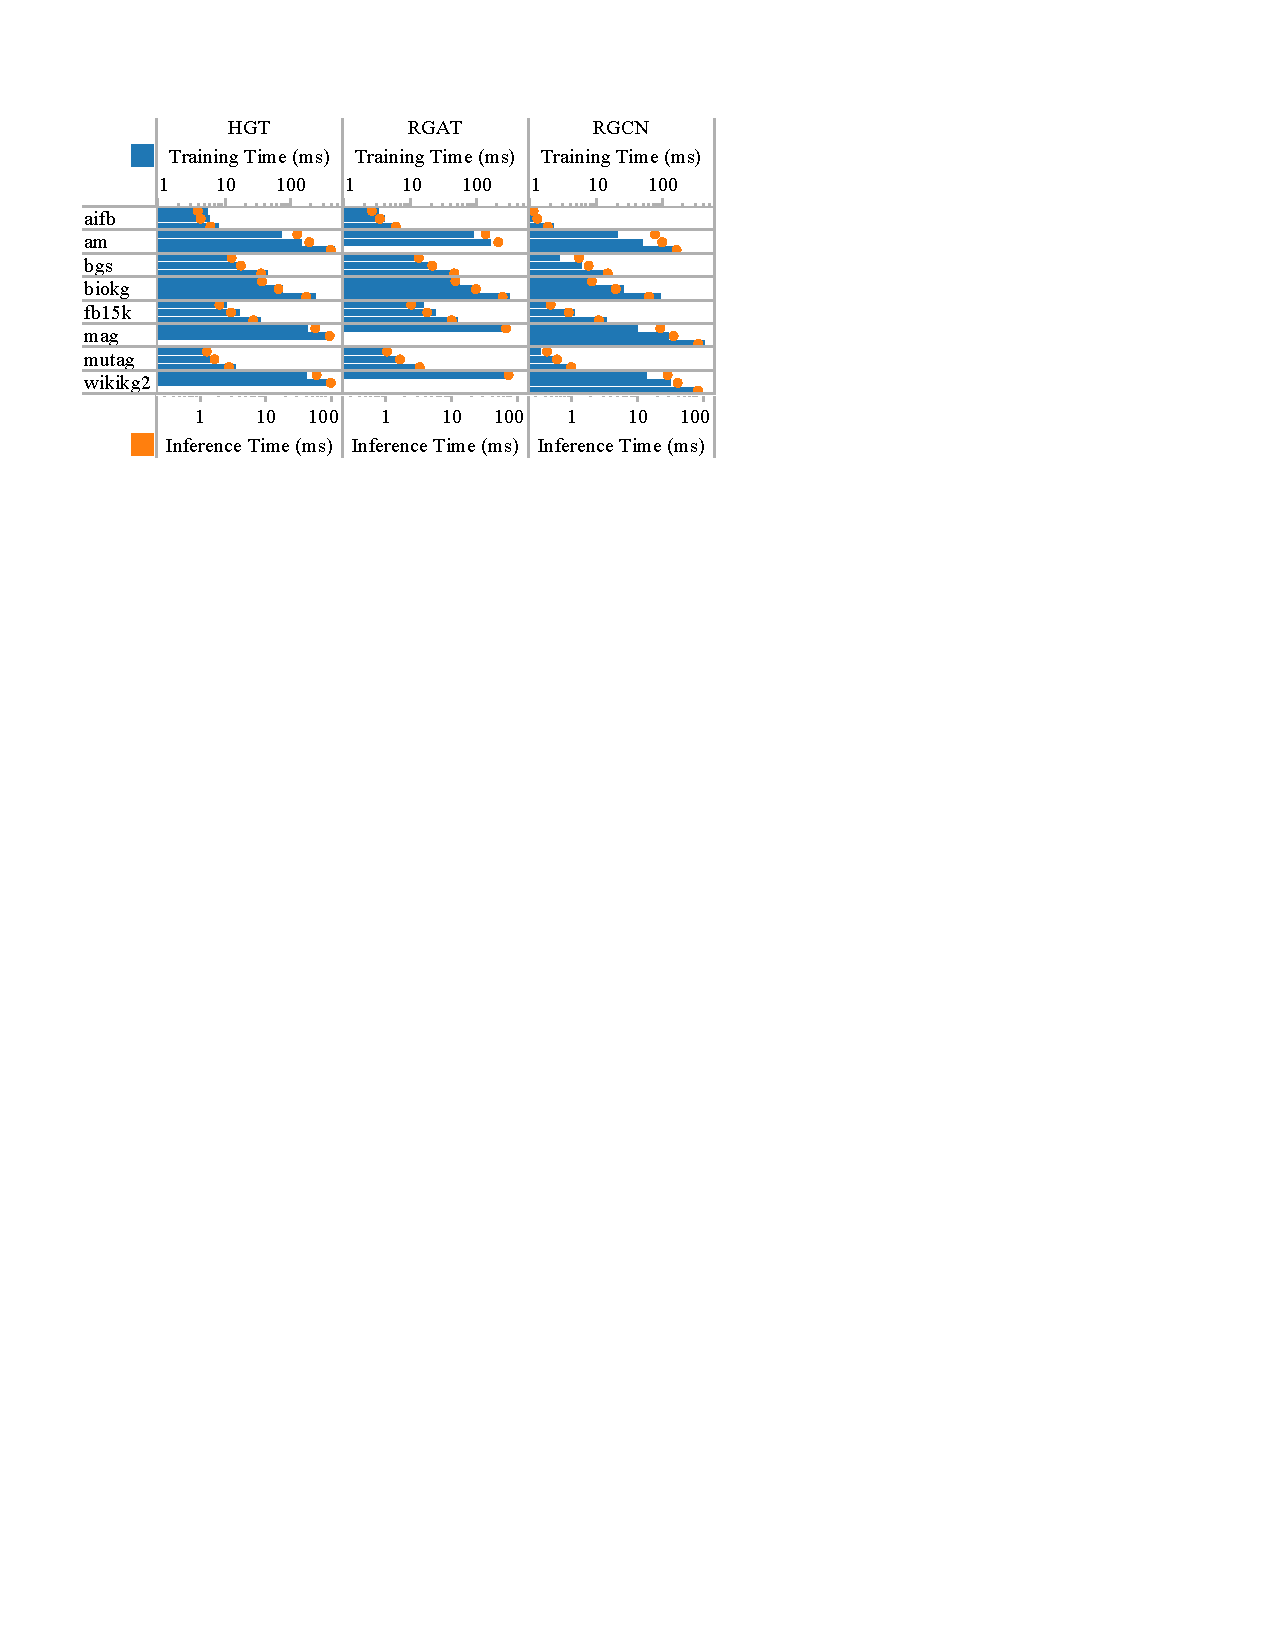
\includegraphics[width=\linewidth]{figures/Hector/HeteroRGNNPerfCurve.pdf}
\caption{\label{fig:perf_curve}Hector unoptimized performance. Each cell corresponds to one pair of dataset and model, where it is shown the time of (input dimension, output dimension) as (32, 32), (64, 64), and (128, 128) from the top to the bottom. Vacancy indicates OOM errors.}
\end{figure}


The instruction per cycle~(IPC) charts in Figure~\ref{fig:arch_number} indicate the traversal kernels are generally latency-bound: on RTX 3090, IPC is ideally four as each SM has four schedulers. Backward propagation kernels have lower throughput due to worsened latency and increased memory bandwidth consumption by doubled memory accesses compared to forward propagation. In backward propagation, backward traversal kernels compute gradients using atomic updates, therefore hindering the throughput; GEMM kernels also, on average, have lower performance due to outer products that compute the delta of weights.





\begin{figure}[!htbp]
\centering
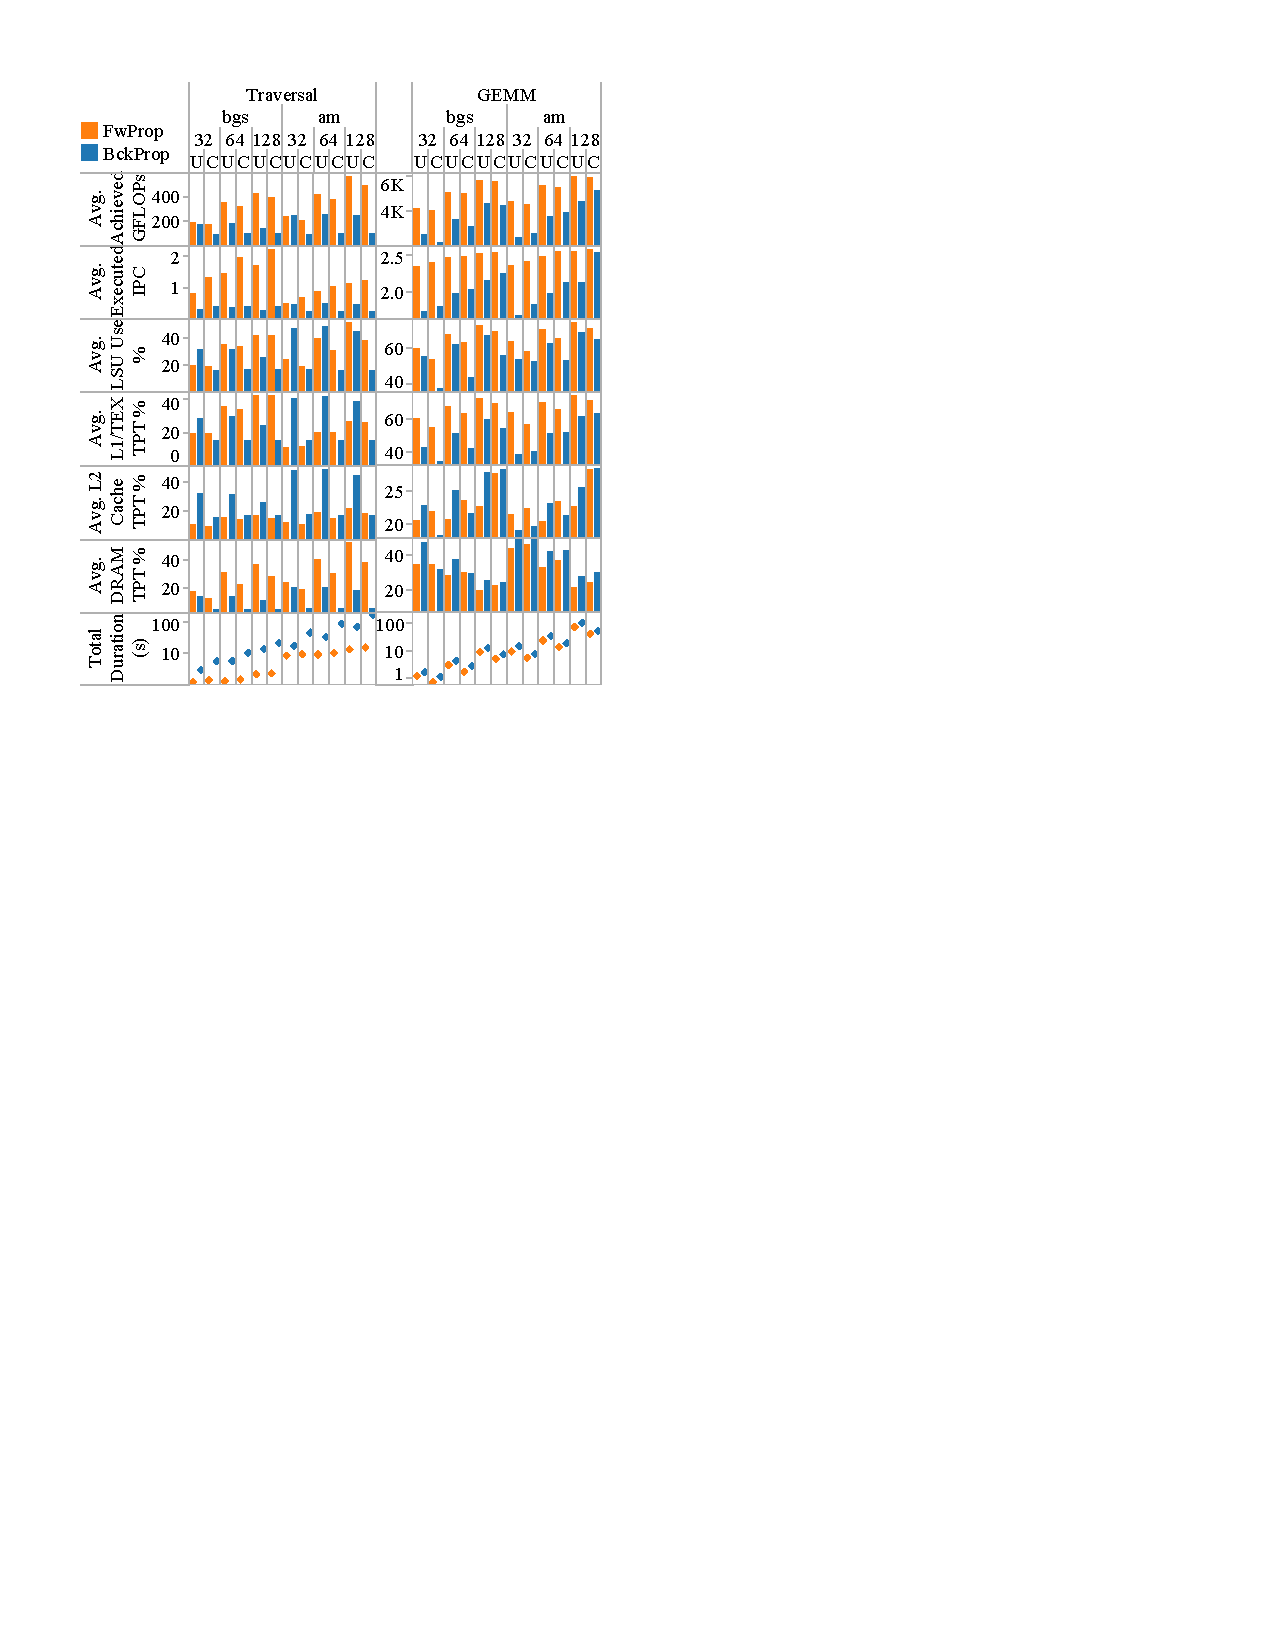
\includegraphics[width=0.8\linewidth]{figures/Hector/upd6_Aggregated.HGT.AM.MAG.Arch_number_portrait_fw_bw_compact.pdf}
\caption{\label{fig:arch_number}Architectural metrics of Hector kernels in the forward~(Fw) and backward~(Bck) propagation when running Hector on RGAT with compaction~(C) and without~(U). For each kernel category, aggregated duration and average~(Avg.) metrics, e.g., instructions per cycle~(IPC) and various throughputs~(TPT), are reported.}
\end{figure}






